% Shared preamble for the English summaries in this repository.
\documentclass[11pt,a4paper]{article}
\usepackage[margin=2.2cm]{geometry}
\usepackage[T1]{fontenc}
\usepackage[utf8]{inputenc}
\usepackage{lmodern}
\usepackage{amsmath,amssymb}
\usepackage{graphicx}
\usepackage{booktabs}
\usepackage{enumitem}
\usepackage[hidelinks]{hyperref}
\setlist{itemsep=2pt,topsep=4pt}
\setlength{\parindent}{0pt}
\setlength{\parskip}{5pt}
\graphicspath{{figures/}}
\newcommand{\summaryheader}[3]{%
  \begin{center}
    {\Large\bfseries #2}\\[3pt]
    {\large #1}\\[3pt]
    {\small Arshia Goshtasbi \textbullet{} MSc Electrical Engineering (Control), Iran University of Science and Technology \textbullet{} #3}
  \end{center}
  \vspace{2pt}\hrule\vspace{8pt}
  \noindent\textit{English summary of my original Persian report, which is kept as a PDF in this folder.}\par}

\begin{document}
\summaryheader{Adaptive Control, Homework 1}{Least-squares Parameter Estimation (Åström \& Wittenmark, Example 2.1)}{Autumn 1404 (2025)}

\section*{Problem}
Seven input--output pairs, $u=0,\dots,6$ and $y=(1,\ 2,\ 2.2,\ 3.5,\ 4.6,\ 6.1,\ 7.8)$, are fitted with polynomial models of order 0 to 3, $y=b_0+b_1u+\dots+b_3u^3$, by least squares: $\hat\theta=(\Phi^T\Phi)^{-1}\Phi^Ty$.

\section*{Results (\texttt{main.m}, re-run in R2023b)}
The loss is $V=\tfrac12\sum_i(y_i-\hat y_i)^2$.
\begin{center}
\begin{tabular}{lcccccc}\toprule
Model & $b_0$ & $b_1$ & $b_2$ & $b_3$ & $V$\\\midrule
Order 0 & 3.8857 & & & & 17.8043\\
Order 1 & 0.5643 & 1.1071 & & & 0.6436\\
Order 2 & 1.1357 & 0.4214 & 0.1143 & & 0.0950\\
Order 3 & 1.0857 & 0.5881 & 0.0393 & 0.0083 & 0.0875\\\bottomrule
\end{tabular}
\end{center}
\begin{center}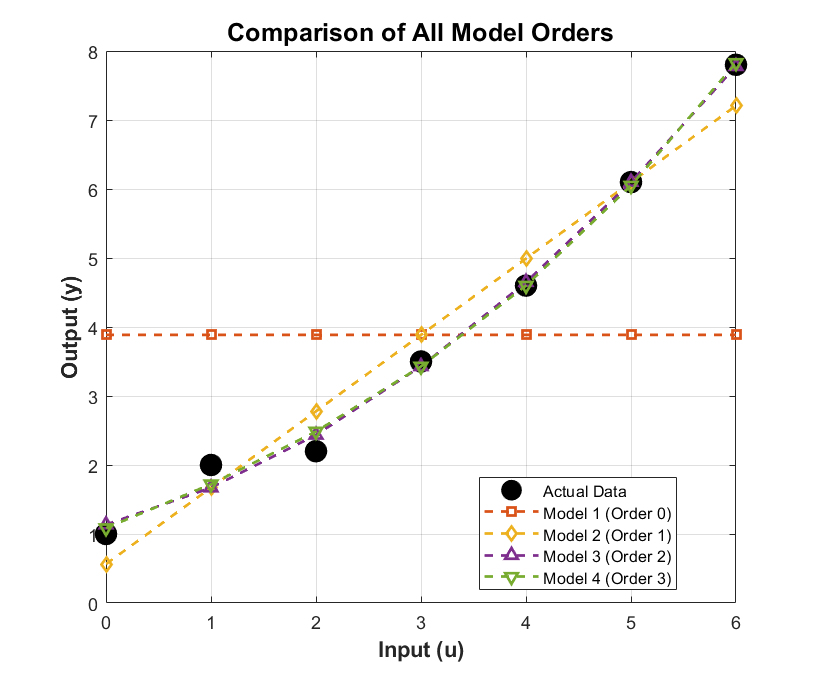
\includegraphics[width=0.55\linewidth]{main_5.png}\end{center}

\section*{Conclusion}
The loss drops sharply from order 0 to order 2 and only slightly after that. Order 1 already captures the trend, and order 2 fits almost exactly. Going to order 3 adds a parameter for very little gain, so model order has to be traded off against the risk of over-fitting.
\end{document}
